\documentclass[a4paper, 12pt]{report}
\usepackage[vietnamese]{babel}
\usepackage{fontspec}
\usepackage{geometry}
\geometry{top=25mm,bottom=25mm,left=25mm,right=25mm}
\usepackage[backend=biber, style=numeric, sorting=none]{biblatex}
\DeclareDelimFormat{multinamedelim}{\addcomma\space}
\DeclareDelimFormat{finalnamedelim}{\space và\space}
\renewbibmacro{in:}{\addsemicolon\space}

\DeclareFieldFormat{pages}{#1}
\DeclareLanguageMapping{vietnamese}{english}
% \DefineBibliographyStrings{english}{
%   andothers = {\textit{et al.}} % In nghiêng et al.
% }

\DeclareFieldFormat{volume}{\textbf{#1}}
\DeclareFieldFormat{number}{(#1)}
\renewbibmacro*{volume+number+eid}{%
  \printfield{volume}%
  \printfield{number}%
  \setunit{\addcomma\space}%
}

\addbibresource{references.bib}

\usepackage{tikz}
\usetikzlibrary{shapes.geometric, arrows, positioning}

\usepackage{siunitx}
\sisetup{
    output-decimal-marker = {,}, % Dấu phẩy thập phân (kiểu VN/Pháp)
    group-minimum-digits = 4,     % Chỉ phân cách khi có từ 4 chữ số trở lên
    list-final-separator = { và },
    range-phrase = { đến }
}

\usepackage{graphicx}
\graphicspath{{imgs/}} % Khai báo thư mục chứa ảnh

\title{Nghiên cứu và thiết kế hệ thống thu âm thanh ứng dụng giao thức truyền thông công nghiệp RS485}
\author{Họ và tên sinh viên}
\date{Tháng 5, 2026}

\begin{document}
\maketitle

\begin{abstract}
Bản báo cáo trình bày nghiên cứu và thiết kế hệ thống thu âm thanh sử dụng giao thức truyền thông công nghiệp RS485. Nội dung bao gồm phân tích yêu cầu, lựa chọn phần cứng và phần mềm, cấu trúc hệ thống, thiết kế mạch, giải pháp truyền dữ liệu và kết quả thử nghiệm.
\end{abstract}

\tableofcontents
\listoffigures
\listoftables

\chapter{Giới thiệu}

\ 

Trong sự phát triển mạnh mẽ của cuộc cách mạng công nghiệp 4.0, các hệ thống truyền tin và cảm biến đóng vai trò là những thành phần cốt lõi trong quy trình vận hành tự động hóa. Nhu cầu về giao tiếp âm thanh và giám sát tại hiện trường trong môi trường công nghiệp ngày càng trở nên cấp thiết \cite{Li2025}. Việc phân tích dữ liệu âm thanh không chỉ giúp giám sát trạng thái hoạt động của máy móc mà còn hỗ trợ trong việc phát hiện sớm sự cố kỹ thuật dựa trên các thuật toán nhận diện âm thanh bất thường.

Tuy nhiên, việc truyền tải tín hiệu âm thanh gặp phải nhiều thách thức về mặt kỹ thuật. Tín hiệu âm thanh tương tự thường bị suy hao trên đường dây dài và đặc biệt nhạy cảm với nhiễu điện từ phát ra từ động cơ, biến tần và thiết bị công suất lớn trong nhà máy \cite{Whitlock2005}. Các giải pháp truyền thông không dây mặc dù có tính linh hoạt cao nhưng lại bộc lộ hạn chế về độ ổn định khi gặp vật cản kim loại hoặc hiện tượng chồng lấn sóng trong môi trường công nghiệp phức tạp. 

Do đó, việc nghiên cứu một phương thức truyền dẫn âm thanh có dây bền bỉ, có khả năng chống nhiễu và truyền tin ở khoảng cách xa là một yêu cầu thực tiễn quan trọng. Giao thức RS485 với đặc tính truyền dẫn vi sai đã chứng minh được hiệu quả vượt trội trong việc loại bỏ nhiễu chế độ chung và duy trì tính toàn vẹn của dữ liệu ở khoảng cách lên tới 1200m \cite{tao2026research}. Đề tài \textbf{“Nghiên cứu và thiết kế hệ thống thu âm thanh ứng dụng giao thức truyền thông công nghiệp RS485”} được thực hiện nhằm giải quyết yêu cầu nêu trên.

\section{Mục tiêu và phạm vi nghiên cứu}
\subsection{Mục tiêu nghiên cứu}
Đề tài tập trung vào việc đạt được những mục tiêu cụ thể sau:
\begin{itemize}
    \item Nghiên cứu cơ chế truyền dẫn của giao thức RS485 và kĩ thuật số hóa tín hiệu âm thanh.
    \item Thiết kế và chế tạo mạch điện tử tích hợp bộ phận cấp nguồn, bộ phận thu âm thanh và bộ xử lí và truyền tải tín hiệu.
    \item Xây dựng giải pháp đóng gói dữ liệu âm thanh để truyền tải qua môi trường RS485.
    \item Thử nghiệm và đánh giá chất lượng âm thanh thu được tại đầu nhận.
\end{itemize}

\subsection{Phạm vi nghiên cứu}
\begin{itemize}
    \item \textbf{Về phần cứng:} Thiết kế bảng mạch in (PCB) cho hệ thống thu âm thanh, sử dụng vi điều khiển phổ biến và các linh kiện điện tử tiêu chuẩn.
    \item \textbf{Về môi trường:} Thử nghiệm hệ thống trong phạm vi truyền dẫn ngắn với tốc độ baud phù hợp để đảm bảo băng thông cho âm thanh.
    \item \textbf{Về chức năng:} Hệ thống tập trung vào việc thu, truyền và tái tạo âm thanh cơ bản.
\end{itemize}

\section{Phương pháp thực hiện}
Để hoàn thành được mục tiêu đề ra, nghiên cứu được triển khai theo các bước như sau:
\begin{enumerate}
    \item \textbf{Nghiên cứu lý thuyết:} Tổng hợp một số tài liệu về tiêu chuẩn RS485, lý thuyết xử lý tín hiệu số hóa và kĩ thuật chống nhiễu cho hệ thống âm thanh.
    \item \textbf{Thiết kế:} Sử dụng phần mềm EasyEDA để thiết kế sơ đồ nguyên lí và sơ đồ mạch in của thiết bị.
    \item \textbf{Thực nghiệm:} Tiến hành lắp ráp mô hình thực tế, lập trình cho vi điều khiển và viết giao diện giao tiếp với người dùng.
   %  \item \textbf{Phương pháp phân tích và đánh giá:} Sử dụng các thiết bị đo lường (Oscilloscope) để kiểm tra dạng sóng và phần mềm phân tích phổ âm thanh để đánh giá độ méo tiếng và tỉ số tín hiệu trên nhiễu (SNR).
\end{enumerate}

\chapter{Cơ sở lý thuyết}

\section{Cấu trúc chung của một thiết bị đo}

\ 

Một hệ thống đo lường và thu thập dữ liệu hiện đại, đặc biệt là các hệ thống ứng dụng trong công nghiệp, thường được cấu tạo từ các khối chức năng cơ bản nhằm biến đổi đại lượng vật lý cần đo thành thông tin định lượng dưới dạng số. Cấu trúc tổng quát của hệ thống được thể hiện qua sơ đồ khối dưới đây:

\begin{figure}[ht]
    \centering
    \begin{tikzpicture}[
        node distance=1.6cm and 2cm,
        block/.style={rectangle, draw, fill=blue!5, text width=2.5cm, align=center, minimum height=1.2cm, font=\small\bfseries},
        arrow/.style={-stealth, thick}
    ]
        % Các khối
        \node (input) [text width=2cm, align=center] {Đại lượng vật lý};
        \node (sensor) [block, right=of input] {Cảm biến};
        \node (signal) [block, right=of sensor] {Chuẩn hóa tín hiệu};
        \node (adc) [block, below=of signal] {Bộ biến đổi ADC};
        \node (processing) [block, left=of adc] {Vi xử lý};
        \node (output) [block, left=of processing] {Giao tiếp \\ và hiển thị};

        % Các mũi tên kết nối
        \draw [arrow] (input) -- (sensor);
        \draw [arrow] (sensor) -- (signal);
        \draw [arrow] (signal) -- (adc);
        \draw [arrow] (adc) -- (processing);
        \draw [arrow] (processing) -- (output);
        
        % Chú thích luồng dữ liệu
        \node at ([xshift=1cm, yshift=0.3cm]sensor.east) {\scriptsize Tín hiệu điện};
        \node [align=center] at  ([xshift=0.8cm, yshift=-0.8cm]signal.south) {\scriptsize Tín hiệu\\[-4pt] \scriptsize tương tự};
        \node at ([xshift=-1cm, yshift=0.3cm]adc.west) {\scriptsize Tín hiệu số};
    \end{tikzpicture}
    \caption{Sơ đồ khối cấu trúc chung của một hệ thống đo lường}
    \label{fig:block_diagram}
\end{figure}

Dựa trên sơ đồ khối trên, các thành phần chính của hệ thống đo bao gồm:

\begin{enumerate}
   \item \textbf{cảm biến:} 
   Đây là phần tử đầu tiên tiếp xúc với đại lượng cần đo. Cảm biến có nhiệm vụ biến đổi đại lượng vật lý thành đại lượng điện mang thông tin của đại lượng cần đo. 
   
   \item \textbf{Chuẩn hóa tín hiệu:} 
   Tín hiệu điện sau khi rời khỏi cảm biến sẽ được đưa vào khối này để được biến đổi thành tín hiệu điện áp. Kết quả sau khối này là một tín hiệu tương tự đã được tối ưu hóa về mặt biên độ và chất lượng.
   
   \item \textbf{Biến đổi tương tự sang số (ADC --- Analog-to-Digital Converter):} 
   ADC thực hiện quá trình lấy mẫu và lượng tử hóa để biến đổi tín hiệu tương tự liên tục thành chuỗi dữ liệu tín hiệu số để có thể đưa vào vi xử lý.

   \item \textbf{Vi xử lý:} 
   Sau khi tiếp nhận dữ liệu số từ bộ ADC, vi xử lý thực hiện các thuật toán biến đổi tín hiệu, đóng gói dữ liệu và điều khiển luồng dữ liệu truyền đi.
   
   \item \textbf{Giao tiếp và hiển thị:} 
   Kết quả đo sau khi xử lý sẽ được truyền đến các thiết bị giám sát (PC, PLC) thông qua chuẩn giao tiếp được định sẵn hoặc hiển thị trực tiếp lên màn hình LCD/OLED. 
    
\end{enumerate}


\section{Các thành phần thu và xử lý âm thanh}

\subsection{Cảm biến thu âm thanh}

\ 

Trong hệ thống này, loại cảm biến được sử dụng là mi-crô tụ điện có phân cực CZN-15E với kích thước nhỏ gọn và độ nhạy cao.

\begin{figure}[ht]
   \centering
   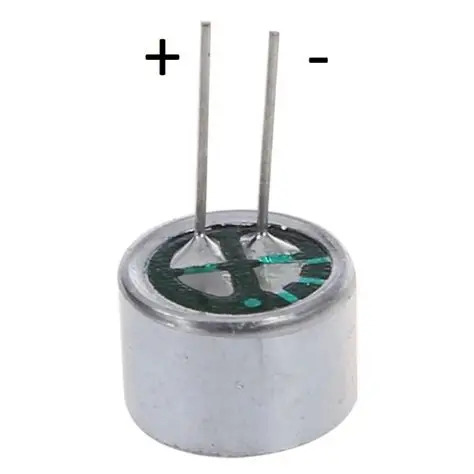
\includegraphics[width=0.4\textwidth]{CZN-15E.jpg} 
   \caption{Cảm biến âm thanh CZN-15E}
   \label{fig:czn15e}
\end{figure}

Các đặc tính kỹ thuật chi tiết của cảm biến được tổng hợp trong Bảng \ref{tab:specs_mic}\cite{czn15e_datasheet}:

\begin{table}[ht]
   \centering
   \caption{Thông số kỹ thuật của cảm biến âm thanh CZN-15E}
   \label{tab:specs_mic}
   \begin{tabular}{|l|l|}
      \hline
      \textbf{Thông số} & \textbf{Giá trị chi tiết} \\ \hline
      Mã hiệu & CZN-15E (Electret Condenser Microphone) \\ \hline
      Kích thước (Đường kính $\times$ Chiều cao) & $\num{9.7}$ mm $\times$ $\num{6.7}$ mm \\ \hline
      Khoảng cách chân cắm & $\num{2.5}$ mm \\ \hline
      Điện áp hoạt động & $\num{1.5}$ V -- $\num{10.0}$ V \\ \hline
      Độ nhạy & $-42 \pm 3$ dB \\ \hline
      Dải tần số đáp ứng & $\num{50}$ Hz -- $\num{16000}$ Hz \\ \hline
      Trở kháng đầu ra & $\num{2.2}$ k$\Omega$ \\ \hline
      Kiểu thu âm & Đa hướng \\ \hline
   \end{tabular}
\end{table}

\subsection{Mạch tiền khuếch đại âm thanh (MAX4466)}

\ 

Tín hiệu điện áp từ microphone tụ điện thường rất nhỏ (cấp mV) và có trở kháng cao, không đủ biên độ để bộ biến đổi ADC xử lý một cách chính xác. Do đó, hệ thống sử dụng IC MAX4466 --- khuếch đại thuật toán công suất thấp --- được tối ưu hóa chuyên biệt cho các ứng dụng thu âm thanh \cite{max4466_datasheet}.

Các đặc tính điện học của MAX4466 giúp nó trở thành lựa chọn lý tưởng cho các hệ thống thu âm chạy pin hoặc lấy nguồn từ bus vi điều khiển trong môi trường công nghiệp. Các thông số quan trọng được tổng hợp trong Bảng \ref{tab:specs_max4466}:

\begin{table}[ht]
    \centering
    \caption{Thông số kỹ thuật của bộ tiền khuếch đại MAX4466}
    \label{tab:specs_max4466}
    \begin{tabular}{|l|l|}
        \hline
        \textbf{Thông số} & \textbf{Giá trị kỹ thuật} \\ \hline
        Điện áp nguồn cung cấp ($V_{CC}$) & \qtyrange{2,4}{5,5}{V} \\ \hline
        Dòng tiêu thụ ($I_{CC}$) & \qty{24}{\micro\ampere} (Điển hình) \\ \hline
        Băng thông tích hệ số khuếch đại (GBWP) & \qty{600}{kHz} (với $A_V \ge 5$) \\ \hline
        Tỷ lệ nén nhiễu nguồn (PSRR) & \qty{112}{dB} \\ \hline
        Tỷ lệ nén nhiễu chế độ chung (CMRR) & \qty{126}{dB} \\ \hline
        Độ lợi vòng hở ($A_{VOL}$) & \qty{125}{dB} \\ \hline
        Kiểu đầu ra (Output Stage) & Rail-to-Rail \\ \hline
        Kiểu đóng gói & 5-Pin SC70 / SOT23 \\ \hline
    \end{tabular}
\end{table}

\subsection{Vi xử lý ESP32-S3}

\ 

Để đáp ứng yêu cầu xử lý tín hiệu âm thanh thời gian thực và quản lý giao thức truyền thông công nghiệp, hệ thống sử dụng vi xử lý \textbf{ESP32-S3}. Đây là dòng SoC (System on Chip) mạnh mẽ của Espressif Systems, được thiết kế chuyên biệt cho các ứng dụng IoT tích hợp trí tuệ nhân tạo và xử lý tín hiệu số (DSP) \cite{esp32s3_datasheet}.

\begin{figure}[ht]
   \centering
   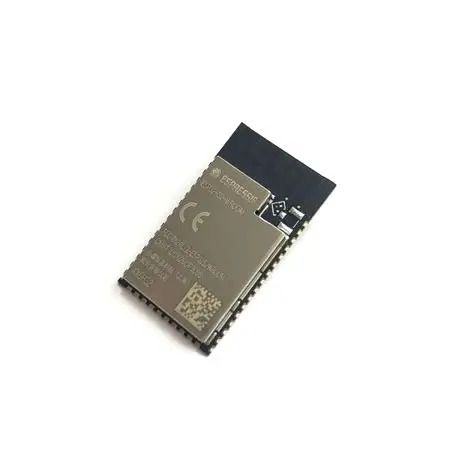
\includegraphics[width=0.5\textwidth]{ESP32-S3.jpg} 
   \caption{Vi xử lý ESP32-S3}
   \label{fig:esp32s3}
\end{figure}

Trái tim của ESP32-S3 là vi xử lý Xtensa® LX7 hai nhân (dual-core) 32-bit với xung nhịp cao. Điểm đặc biệt của dòng chip này so với các thế hệ trước là việc tích hợp bộ lệnh mở rộng (PIE). Bộ lệnh này hỗ trợ tăng tốc các phép toán vector và ma trận, vốn là nền tảng trong các thuật toán lọc số và nén dữ liệu âm thanh.

ESP32-S3 sở hữu bộ nhớ nội bộ (SRAM) lớn cùng khả năng mở rộng bộ nhớ ngoài (PSRAM) qua giao tiếp tốc độ cao, giúp hệ thống không bị mất mát thông tin khi xảy ra hiện tượng chiếm dụng bus truyền thông hoặc khi vi xử lý đang thực hiện các tác vụ tính toán nặng.

Ngoài ra, ESP32-S3 tích hợp đầy đủ các tính năng cần thiết cho các ứng dụng công nghiệp, bao gồm:
\begin{itemize}
    \item \textbf{Khối biến đổi tương tự - số (ADC):} Bộ ADC 12-bit tích hợp cho phép số hóa tín hiệu với độ phân giải cao.
    \item \textbf{Quản lý năng lượng:} Chip hỗ trợ nhiều chế độ tiết kiệm điện thông minh, phù hợp cho các thiết bị giám sát tại hiện trường vốn cần hoạt động bền bỉ và ổn định.
\end{itemize}

\section{Giao thức truyền thông công nghiệp RS485}

\ 

RS485 (hay TIA/EIA-485) là một tiêu chuẩn giao tiếp vật lý được thiết kế cho các ứng dụng truyền dữ liệu nối tiếp trong môi trường có độ nhiễu điện từ cao và khoảng cách truyền dẫn dài \cite{tao2026research}. Sự bền bỉ của RS485 đến từ cơ chế truyền dẫn và cấu trúc mạng đặc thù.

\subsection{Cơ chế truyền tín hiệu vi sai}

\ 

Đặc điểm cốt lõi của RS485 là sử dụng phương pháp truyền tín hiệu vi sai (differential signaling) trên hai dây dẫn xoắn đôi, ký hiệu là dây A (hay dây không đảo --- non-inverting) và dây B (hay dây đảo --- inverting). Khác với các chuẩn như RS232 sử dụng điện áp so với nguồn đất chung (GND), RS485 xác định trạng thái lô-gích dựa trên sự chênh lệch điện áp giữa hai dây:
\begin{equation}
   U_{AB} = V_A - V_B
\end{equation}
Theo tiêu chuẩn kỹ thuật:
\begin{itemize}
   \item Nếu $U_{AB} > +200$ mV: Bộ thu nhận dạng mức lô-gích 1 (Mark).
   \item Nếu $U_{AB} < -200$ mV: Bộ thu nhận dạng mức lô-gích 0 (Space).
\end{itemize}

\subsection{Khả năng chống nhiễu chế độ chung}

\ 

Trong môi trường công nghiệp, nhiễu điện từ thường tác động lên cả hai dây dẫn. Nhờ đặc tính dây xoắn đôi, thành phần nhiễu ($\Delta V$) tác động lên dây A và B là gần như tương đồng. Tại đầu thu, phép toán hiệu số sẽ triệt tiêu thành phần nhiễu này:
\begin{equation}
   U_{AB\_new} = (V_A + \Delta V) - (V_B + \Delta V) = V_A - V_B = U_{AB}
\end{equation}
Kết quả là tín hiệu hữu ích vẫn được bảo toàn ngay cả khi có sự hiện diện của nhiễu biên độ lớn. Ngoài ra, giao thức này cho phép kết nối đa điểm (multi-drop) với tối đa 32 thiết bị trên cùng một đường và khoảng cách truyền dẫn có thể đạt tới 1200 mét.




\printbibliography[title={Tài liệu tham khảo}]
\end{document}